\chapter{Endocrine System (Glands)}
\label{chap:Endocrine-System}
\label{chap:Glands}

An {\bf endocrine system} (Greek: {\it endo}- = inside, {\it krinein} = to
separate, to distinguish), is a collection of {\bf glands} in the (1) brain, (2)
body of an organism that \textcolor{red}{secretes hormones {\bf directly} into
the circulatory system to be carried toward distant target organs to regulate
its function.} The endocrine system's effects are slow to initiate, and
prolonged in their response, lasting from a few hours up to weeks.
This is in opposite to the nervous system (Chap.\ref{chap:nerve-signals}) which
sends information very quickly, and responses are generally short lived.
\textcolor{red}{Hormonal effects take effect slower, yet can last up to ten
times longer than those of neurotransmitters}. 
However, recent findings indicate that this may not actually be the case.
\url{https://www.nature.com/articles/ncomms12620}
\url{https://www.sciencedaily.com/releases/2016/11/161114081911.htm}

The nervous system and endocrine system is connected via neuroendocrine cells
(Sect.\ref{sec:neuroendocrine-cell}).
NOTE: {\bf Neuroendocrinology} is the study of the interaction between the
nervous system (Chap.\ref{chap:CNS}) and the endocrine system.
The major center of neuroendocrine integration in the body is found in the
hypothalamus and the pituitary gland (Sect.\ref{sec:pituitary-gland}).
Neuroendocrinology arose from the recognition that the brain, especially the
hypothalamus (Sect.\ref{sec:hypothalamus}), controls secretion of pituitary
gland hormones (Sect.\ref{sec:glands-head-neck}).

\begin{itemize}
  \item When cell membrane proteins on one cell surface interact with receptor
  proteins on adjacent cell surfaces, these events are called {\bf juxtacrine
  interactions} (since the cell membranes are juxtaposed).

  \item When proteins synthesized by one cell can diffuse over small distances
  to induce changes in neighboring cells, the event is called a {\bf paracrine
  interaction}; and the diffusible proteins are called {\bf paracrine factors}
  (growth and differentiation factors (GDFs)) involved in paracrine signalling
  (Sect.\ref{sec:paracrine-factors}).
  

  \item those that travel far in distance via the circulatory system are called
  {\bf endocrine factors} (or hormones)
  
\end{itemize}

\begin{mdframed}

NOTE: In contrast to endocrine system, the {\bf exocrine system} secretes
its hormones using ducts.
Examples of exocrine glands:  salivary glands, sweat glands, and glands within
the gastrointestinal tract.


\end{mdframed}


\section{Neuropeptides}
\label{sec:neuropeptides}

Neurotransmitters (Sect.\ref{sec:neurotransmitter}) is not the only way that
neurons used to communicate with each other. {\bf Neuropeptides} are small
protein-like molecules (peptides) used by neurons to communicate with each
other. Many neuropeptides are co-released with other small-molecule
neurotransmitters. 


Neuropeptides is a general term describing a large number of peptides that
function as neurotransmitters or neurohormones. Neuropeptides are often released
upon high-stimulus or high elevation of $\Ca$ concentration in axonal terminal.
The human genome contains about 90 genes that encode precursors of
neuropeptides; with more than 100 known different neuropeptides released by
different populations of neurons.
\textcolor{red}{FULL DATABASES}: \url{http://www.neuropeptides.nl/}

Different neuropeptides are involved in a wide range of brain functions,
including analgesia, reward, food intake, metabolism, reproduction, social
behaviors, learning and memory.

\begin{enumerate}
  \item Neuropeptide Y : Sect.\ref{sec:neuropeptide-Y}

\url{http://www.ncbi.nlm.nih.gov/books/NBK10818/}
\end{enumerate}


Neuropeptides modulate neuronal communication by acting on cell surface
receptors. Many neuropeptides are co-released with other neurotransmitters.
Neuropeptides are generally packaged in large dense-core vesicles, and the
co-existing neurotransmitters in small synaptic vesicles.
{\it The large dense-core vesicles are often found in all parts of a neuron,
including the soma, dendrites, axonal swellings (vericosities) and nerve
endings, whereas the small synaptic vesicles are mainly found in clusters at
presynaptic locations}. However, unlike neurotransmitters, one major difference
is that peptides are not
recycled back into the cell once secreted. Release of the large vesicles and the
small vesicles is regulated differently.

{\it Another difference is that after secretion, peptides are modified by
extracellular peptidases; in some cases, these extracellular cleavages
inactivate the biological activity, but in other cases the extracellular
cleavages increase the affinity of a peptide for a particular receptor while
decreasing its affinity for another receptor. These extracellular processing
events add to the complexity of neuropeptides as cell-cell signaling molecules.}




\subsection{Neuropeptide coexists with neurotransmitters}

These neurotransmitters coexist with the folliwng neuropeptides 
\begin{itemize}
  \item norepinephrine neurotransmitter: coexist with
  \begin{verbatim}
Galanin
Enkephalin
Neuropeptide Y
  \end{verbatim}

  \item Epinephrine neurotransmitter: coexist with
  \begin{verbatim}
Neuropeptide Y
Neurotensin  
  \end{verbatim}

  \item Dopamine neurotransmitter: coexist with
  \begin{verbatim}
Cholecystokinin
Neurotensin  
  \end{verbatim}

  \item GABA neurotransmitter: coexist with
  \begin{verbatim}
Somatostatin (in the hippocampus)
Cholecystokinin
Neuropeptide Y (in the arcuate nucleus)  
  \end{verbatim}

  \item Acetylcholine neurotransmitter: coexist with
  \begin{verbatim}
VIP
Substance P  
  \end{verbatim}


  \item Serotonin neurotransmitter: coexist with
  \begin{verbatim}
Substance P
TRH
Enkephalin
  \end{verbatim}

\end{itemize}
\url{https://en.wikipedia.org/wiki/Neuropeptide}


\subsection{Kisspeptins}
\label{sec:kisspeptins}

Neuropeptide {\bf kisspeptin} (encoded by Kiss1 gene,
Sect.\ref{sec:kisspeptins}) and its receptor {\bf Kiss1R} (or GPR54 -
Sect.\ref{sec:GPR54}) have been implicated in pubertal development and adulthood
fertility (Sect.\ref{sec:pubertal-development}), besides their role in cancer
treatment.

\begin{mdframed}

{\bf HISTORY}: Kiss1 - the letters ``{\bf ss}" indicate a ``suppressor sequence"
and ``{\bf Ki}" was added as a prefix to reflect the fact that the molecule was
discovered in Hershey, Pennsylvania, home of the Hershey chocolate ``Kiss"
\citep{lee1996}.

Kiss1 gene were found to suppress metastasis of melanoma and
breast cancer cells, the 54 amino acid protein product of Kiss1
was named {\bf metastin} (aka kisspeptin-54).

It was later shown that kisspeptin-54, as well as shorter fragments
(collectively called kisspeptins), all bind and activate GPR54.

\end{mdframed}

Sex steroids regulate the expression of KiSS-1 mRNA in the brain through direct
action on KiSS-1 neurons. 

\subsection{Neuropeptide Y (NPY)}
\label{sec:neuropeptide-Y}

In the brain, NPY is produced in various locations including the 
paraventricular nucleus (PVN) of the hypothalamus (Sect.\ref{sec:hypothalamus}),
and is thought to have several functions, including: increasing food intake and
storage of energy as fat, reducing anxiety and stress, reducing pain perception,
affecting the circadian rhythm, reducing voluntary alcohol intake, lowering
blood pressure, and controlling epileptic seizures.

NPY receptors are GPCR (Sect.\ref{sec:G-protein-coupled-receptor})
\begin{itemize}
  \item Y1 receptor + Y5 receptor

By blocking these receptors, it reduces foot intake.
  
  \item Y2 receptors + Y4 receptor
  
  To have roles in appetite inhibition (satiety)
\end{itemize}


\section{Hormones}
\label{sec:hormones}

\subsection{somatostatin (GHIH)}
\label{sec:somatostatin}
\label{sec:GHIH}

Somatostatin, also known as growth hormone-inhibiting hormone (GHIH), is a
peptide hormone that regulates the endocrine system and affects
neurotransmission and cell proliferation via interaction with
G-protein coupled somatostatin receptor.

Release of somatostatin is induced by low pH.
By increasing the release of somatostatin, it reduces the rate of secretion of
growth hormone. Upon released and binding to GPCR, somatostatin inhibits insulin
and glucagon secretion in the target cells.

Among vertebrate, there are maximum 6 genes (SS1, SS2, SS3, SS4, SS5, SS6)
expressed somatostatin, and 5 different G-protein coupled somatostatin
receptors. This allows somatostatin to possess a large range of functions.
Zebrafish express all six genes. \textcolor{red}{Humans have only one
somatostatin gene, SST}.

Neurons that produce somatostatin are somatostatin-like neurons
(Sect.\ref{sec:somatostatin-containing-interneuron}).


\subsection{Antidiuretic hormone (ADH) }
\label{sec:antidiuretic-hormone}
\label{sec:ADH}

\subsection{neurohypophysial hormones: vasopressin, oxytocin}
\label{sec:hormone-neurohypophysial-hormones}
\label{sec:vasopressin}
\label{sec:oxytocin}

{\bf neurohypophysial hormones} has 2 types
\begin{itemize}
  \item vasopressin (AVP, ADH):
  arginine vasopressin (AVP), antidiuretic hormone (ADH), or argipressin
  
  Its two primary functions are to retain water in the body (acting to increase
  water reabsorption in the kidney's collecting ducts) and to constrict blood
  vessels.
  
  \item  \textcolor{red}{oxytocin} (Oxt): normally produced by  magnocellular
  neurosecretory cells in the hypothalamus
  (Sect.\ref{sec:Magnocellular-neurosecretory-cell}) and then release into the
  blood stream by posterior pituitary (Sect.\ref{sec:pituitary-gland}), but can be available as a medication.
  
  
  It is used to cause contraction of the uterus, which is used to start labor,
  increase the speed of labor, and to stop bleeding following delivery
  
  Oxytocin was discovered by Henry Dale in 1906.[10] Its molecular structure was
  discovered in 1952.
\end{itemize}

\subsection{follicle-stimulating hormone (FSH)}
\label{sec:hormone-FSH}
\label{sec:FSH}

Follicle-stimulating hormone (FSH) is synthesized and secreted by anterior
pituitary gland (Sect.\ref{sec:pituitary-gland}), and regulates the development,
growth, pubertal maturation, and reproductive processes of the body.

{\bf IMPORTANT}: FSH and luteinizing hormone (LH) act synergistically in
reproduction.
\url{https://en.wikipedia.org/wiki/Follicle-stimulating_hormone}

\subsection{Luteinizing hormone (LH)}
\label{sec:luteinizing-hormone}
\label{sec:LH}


Luteinizing hormone (LH) is synthesized and secreted by anterior pituitary gland
(Sect.\ref{sec:pituitary-gland}), and triggers ovulation.   In males, LH
had also been called interstitial cell-stimulating hormone (ICSH).

{\bf IMPORTANT}: FSH and luteinizing hormone (LH) act synergistically in
reproduction.

\subsection{glucocorticoid hormone}
\label{sec:glucocorticoid-hormone}

{\bf Glucocorticoid hormone} (mainly cortisol in humans) is released from
adrenal cortex upon stimulation of ACTH (Sect.\ref{sec:ACTH}).

\subsection{corticotropin-releasing hormone (CRH)}
\label{sec:CRH}

Name: Corticotropin-releasing hormone (CRH) also known as
corticotropin-releasing factor (CRF) or corticoliberin.

CRH is secreted from paraventricular nucleus of the hypothalamus in response to
stress, and also synthesized from peripheral tissues (e.g. T lymphocytes,
placenta).
Increased CRH production has been observed to be associated with Alzheimer's
disease and major depression.



\subsection{ adrenocorticotropic hormone (ACTH)}
\label{sec:ACTH}

{\bf Adrenocorticotropic hormone} (ACTH), once known as corticotropin, is
released from anterior pituitary gland (Sect.\ref{sec:pituitary-gland}).
 
\subsection{estrogen}
\label{sec:estrogen}

Estrogens or oestrogens are a group of compounds named for their importance in
female sex hormones. However, estrogens have been found to be present in the
blood and urine of males, which suggests they have more uses  than just womanly
curves and reproduction. 
\begin{itemize}
  \item play an important role in heart disease, e.g. CHD
  (Sect.\ref{sec:CHD})
  
  \item play an important role in forming memory:
  \begin{itemize}
    \item  Estrogen is associated with an increase in the release of certain brain
  neurotransmitters. 
  
    \item Estrogen is an important morphogen (Sect.\ref{sec:morphogen}) that
    stimulates brain cell growth in the hypothalamus and hippocampus.
    
    
  \end{itemize}
  
  
  The reduction in estrogen productin in male is gradually; while that in woman
  happens suddenly. In addition,  a female's final estrogen production rate may
  be significantly smaller than a male's.
  The sudden lower estrogen production links to Alzheimer's disease
  (Sect.\ref{sec:Alzheimer-Disease}).
  
\end{itemize}


Types of estrogens:
\begin{itemize}
  \item {\bf natural estrogens}: steroid hormones which include
  (1) sex hormones (e.g. androgens, estrogens, progestagens), 
  (2) corticosteroids
  (3) anabolic steroids
  
  
\begin{mdframed}
A {\bf steroid} is a group of cyclic organic compounds, typically 17 carbon
atoms in a four-ring structure: each first three rings (A, B, C) is composed
of 6 carbon atoms (cyclohexan ring); and the last right (D) is composed of 5
carbon (cyclopentan ring), Fig.\ref{fig:Steroid}.
There are two steroisomeric forms: 5$\alpha$ and 5$\beta$.

When the two methyl groups and 8 carbon side chain (at C-17, as shown for
cholesterol, Fig.\ref{fig:Steroid}(A)) are present, the steroid is said to have
a {\bf cholestane framework}. In cholesterol,  the wedges/lines extending from
C-10, C-13, and C-20 represent methyl groups.

Methyl groups are normally present at C-10 and C-13. An alkyl side chain may
also be present at C-17.  There is a hydroxyl group at C-3 and most of the
skeleton of cholestane.

\url{https://en.wikipedia.org/wiki/Steroid}
\end{mdframed}
  
  \item {\bf synthetic estrogens}: 
\end{itemize}

\begin{figure}[htb]
\centerline{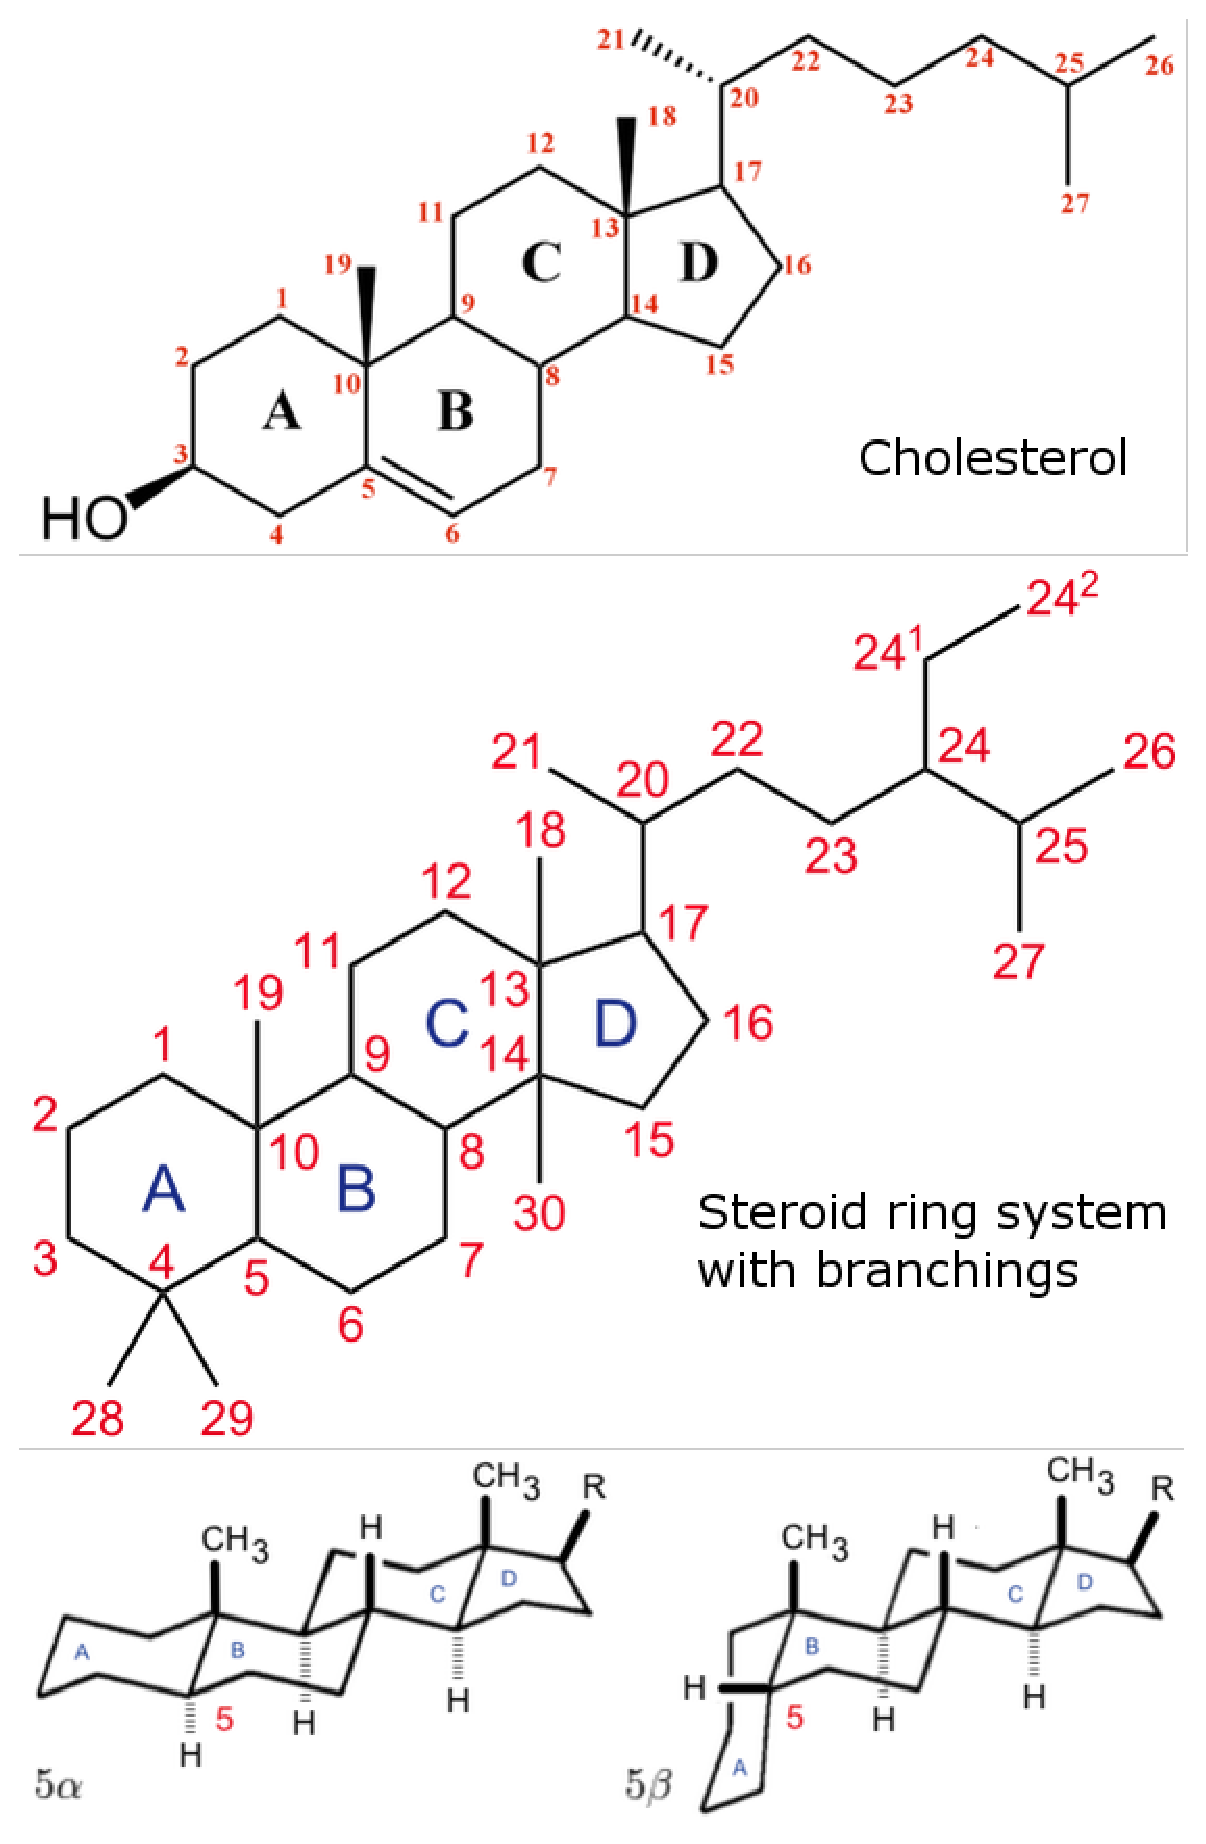
\includegraphics[height=7cm]{./images/Steroid.eps}}
\caption{(A) Cholresterol (Bonds extending above the plane are indicated with
bold wedges, and those extending below the plane with cross-hatched wedges); (B)
Gonane: the simplest steroid with 17-carbon compound}
\label{fig:Steroid}
\end{figure} 

Estrogens are used in (1) oral contraceptives, (2) estrogen replacement therapy
(Sect.\ref{sec:menopause-aging})
Steroids and their metabolites often function as signalling molecules. The most
notable examples are the steroid hormones.

Steroids along with phospholipids function as components of cell membranes. 
Steroids such as cholesterol decrease membrane fluidity, which is a major cause
blood clot in patients with obesity.



\section{Axis}
\label{sec:axis-gland-sequence}

When a number of glands that signal each other in sequence, it is usually
referred to as an axis
\begin{enumerate}
  \item hypothalamic-pituitary-adrenal axis (HPA axis) (Sect.\ref{sec:HPA-axis})
  
   \item hypothalamic-pituitary-gonadal (HPG) axis (Sect.\ref{sec:HPG-axis})
\end{enumerate}

\subsection{Hypothalamic-pituitary-adrenal axis (HPA, HTPA)}
\label{sec:HPA-axis}

NAMES: The hypothalamic-pituitary-adrenal axis (HPA or HTPA axis)
or limbic-hypothalamic-pituitary-adrenal axis (LHPA axis), or
hypothalamic-pituitary-adrenal-gonadotropic axis.


The {\bf hypothalamic-pituitary-adrenal axis} (HPG axis)
refers to the effect of 
\begin{itemize}
  \item hypothalamus (Sect.\ref{sec:hypothalamus})
  which releases  Gonadotropin-releasing hormone (GnRH)
  from  GnRH-expressing neurons (Sect.\ref{sec:GnRH-expressing-neurons})
  
  \item pituitary gland - Sect.\ref{sec:pituitary-gland}
  which releases luteinizing hormone (LH)
  
  \item adrenal cortex - Sect.\ref{sec:adrenal-gland} which releases
  glucocorticoid hormone (Sect.\ref{sec:glucocorticoid-hormone})
  
\end{itemize} 
to control reactions to stress and regulates many body processes,
including digestion, the immune system, mood and emotions, sexuality, and energy
storage and expenditure

 

\subsection{Hypothalamic-pituitary-gonadal (HPG) axis}
\label{sec:HPG-axis}

In oviparous organisms (e.g. fish, reptiles, amphibians, birds), the HPG axis is
commonly referred to as the hypothalamus-pituitary-gonadal-liver axis
(HPGL-axis) in females.


The {\bf hypothalamic-pituitary-gonadal axis} (HPG axis)
refers to the effect of 
\begin{itemize}
  \item hypothalamus (Sect.\ref{sec:hypothalamus})
  which releases  Gonadotropin-releasing hormone (GnRH)
  from  GnRH-expressing neurons (Sect.\ref{sec:GnRH-expressing-neurons})
  
  \item pituitary gland - Sect.\ref{sec:pituitary-gland}
  which releases luteinizing hormone (LH)
  
  \item gonads - Sect.\ref{sec:gonad} 
  which releases estrogen and testoterone.
  
\end{itemize} 
on development, reproduction, and aging.

\url{https://en.wikipedia.org/wiki/Hypothalamic-pituitary-gonadal_axis}

\section{Glands}
\label{sec:glands}

NOTE: A gland is an organ in the human or animal body that secretes particular
chemical substances for use in the body or for discharge into the surroundings.

There are major glands
\begin{enumerate}
  \item pineal gland

  \item pituitary gland - Sect.\ref{sec:pituitary-gland}
  
  \item pancreas
  
  \item ovaries

  \item testes
  
  \item thyroid gland
  
  \item parathyroid gland

  \item hypothalamus (Sect.\ref{sec:hypothalamus}) \textcolor{red}{this is the
  neural control center for all endocrine systems}
  
  \item gastrointestinal tract and 
  
  \item adrenal  glands - Sect.\ref{sec:adrenal-gland}.
\end{enumerate}

There are non-gland organs that also secrete hormones as their secondary
functions
\begin{enumerate}
  \item bone
  
  \item kidney (Chap.\ref{chap:kidney})
  
  \item liver
  
  \item heart
  
  \item gonads
  
\end{enumerate}

\section{-- Glands in head-neck}
\label{sec:glands-head-neck}



There are different glands in the brains and they secretes different hormones,
Fig.\ref{fig:glands-and-their-hormones-in-head-neck}. Hypothalamus plays a
central role as it releases many hormones that involve in the regulating many
other glands.

\begin{figure}[htb]
  \centerline{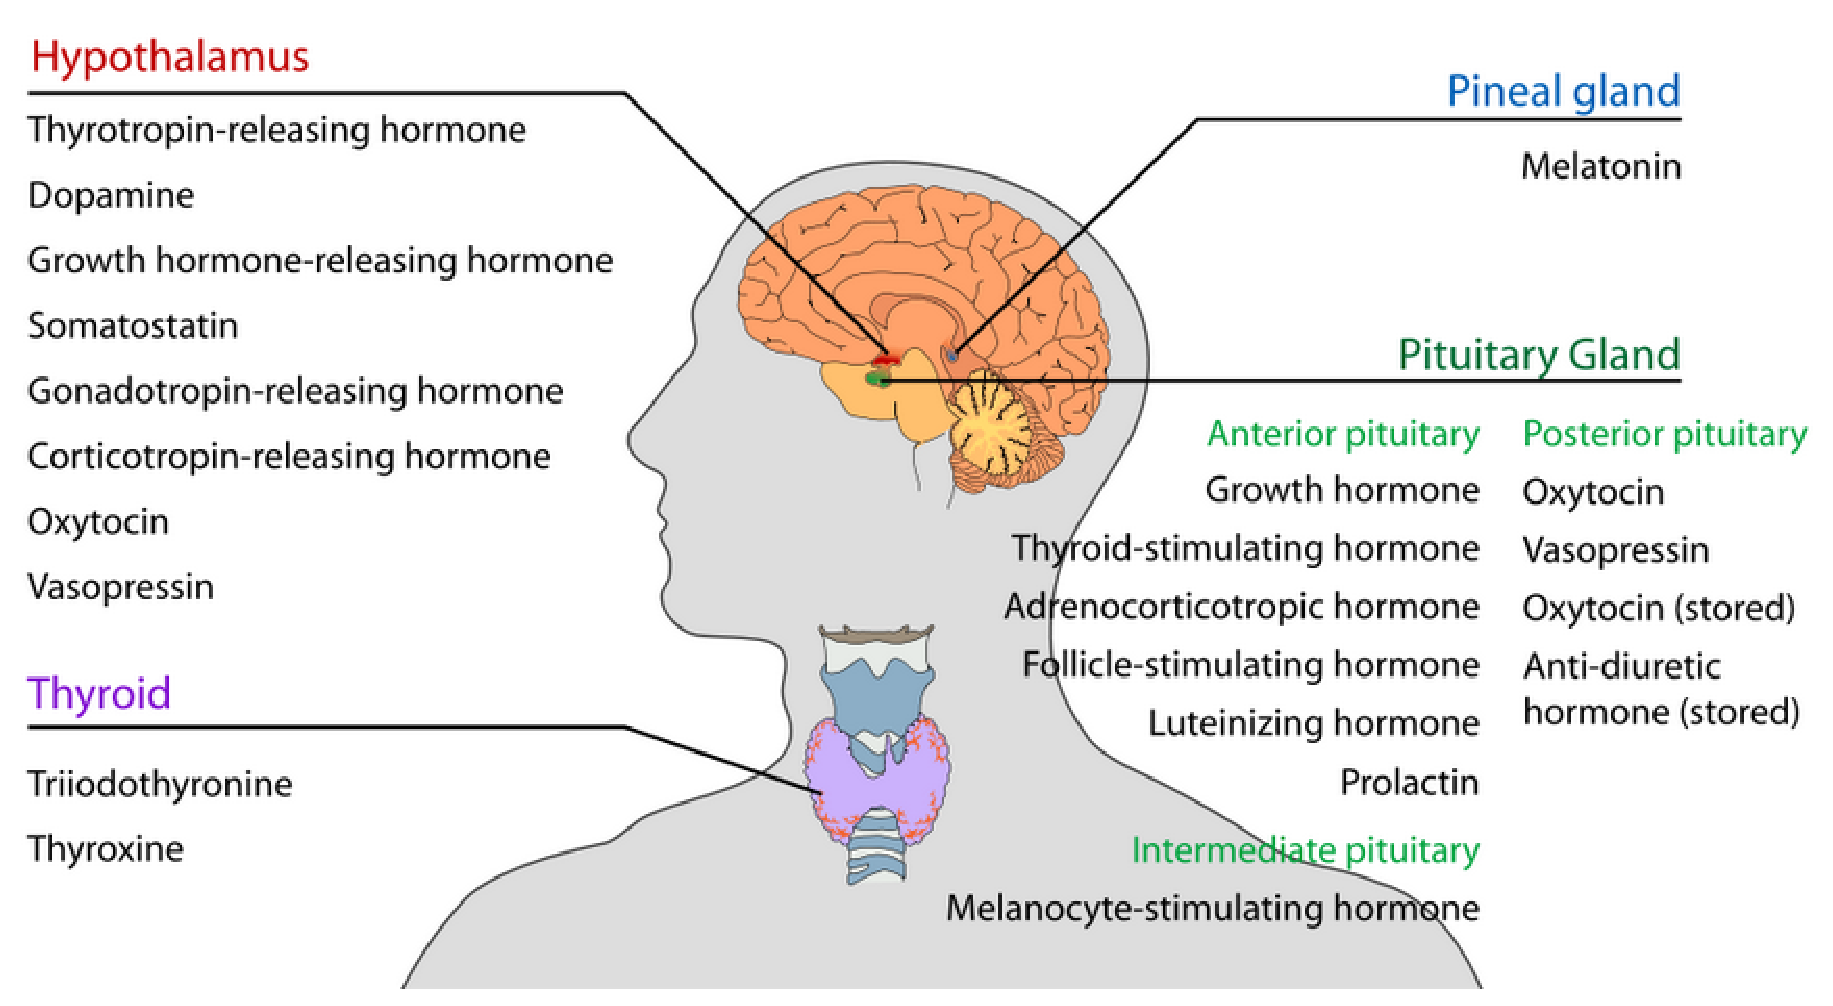
\includegraphics[height=6cm]{./images/glands-and-their-hormones-in-head-neck.eps}}
  \caption{Endocrine glands:
  hypothalamus, pineal gland,
  pituitary gland, thyroid;
  and their hormones}\label{fig:glands-and-their-hormones-in-head-neck}
%https://en.wikipedia.org/wiki/Endocrine_system  
\end{figure}

The hypothalamus communicates with the anterior and posterior {\bf pituitary
gland} to regulate endocrine functions (i.e. secretion of hormones) via 2
pathways:
\begin{enumerate}
  \item direct axonal connections to the {\bf posterior pituitary gland}:
  tuberoinfundibular pathway (Sect.\ref{sec:tuberoinfundibular-pathway}) 
  %(vasopressin and oxytocin control)
  \begin{itemize}
    
    \item {\it anti-diuretic hormone}:  hypothalamus senses the blood osmolality
    (concentration of electrolytes and sodium) and blood pressure, and
    it signals the posterior pituitary to release anti-diuretic hormone, which
    decreases urine output, thus increasing the volume of water in the blood

    \item {\it oxytocin}:  hypothalamus senses stimuli (e.g. stretch of the
    uterus or mechanical stimulation of the nipples), and signals the posterior
    pituitary to release oxytocin, which stimulates uterine contraction and milk
    ejection.
  \end{itemize}
  
  \item release the soluble humoral factors (i.e. hormones) into the
  hypothalamic-hypophyseal portal system (to influence {\bf anterior pituitary
  gland}'s function).
  \begin{itemize}
    
    \item {\bf Growth hormone releasing hormone (GHRH)}: hypothalamus senses
    stress or low blood sugar, and then releases GHRH which then stimulates
    posterior pituitary gland to release growth hormone (this hormone affects
    uptake of amino acids, protein synthesis, as well as promotes bone and cartilage growth.)
    
    \item {\bf thyroid-releasing hormone}: the released hormone stimulates
    thyroid to produce thyroid-stimulating hormone which then causes an
    increased in triiodothyronine (T3) and tetraiodothyronine (T4).
    
    \item {\bf corticotrophin releasing hormone (CRH)}: hypothalamus releases
    CRH under stress or low blood glucose signals. CRH then stimulates anterior
    pituitary gland to release Adrenocorticotropic hormone (ACTH), which target
    the adrenal cortex and stimulates cortisol secretion which results in
    increases in fat, protein degradation and blood glucose, and 
    also has anti-inflammatory effects.
    
    \item {\bf gonadotropin-releasing hormone}: upon releases, it stimulates the
    anterior pituitary gland to secrets luteinizing hormone and
    follicle-stimulating hormone.
    
    \item {\bf prolactin-releasing hormone}: upon releases, it stimulates the
    anterior pituitary to secrete prolactin
    
    \item {\bf prolactin-inhibiting hormone}: upon releases, it reduces the
    production of prolactin from the anterior pituitary glands
  \end{itemize}
 \end{enumerate}
 \footnote{\url{http://www.saylor.org/site/wp-content/uploads/2011/09/BIO303-Subunit6.2.1-ThalamusHypothalamusPrethalamusandEpithalamus-Final.pdf}}

\subsection{Hypothalamus}

Pituitary gland and hypothalamus are the two hormone-release regions in the
brain. Check Sect.\ref{sec:hypothalamus}.

\subsection{Pituitary gland}
\label{sec:pituitary-gland}

Pituitary gland and hypothalamus are the two hormone-release regions in the
brain.

The {\bf pituitary gland} (hypophysis) is composed of three parts, yet in human
the intermediate lobe/gland is but a few cell layers thick and indistinct; as a
result, it is often considered as part of the anterior pituitary
\begin{enumerate} 
  \item anterior pituitary gland - Sect.\ref{sec:anterior-pituitary-gland}
  
  \item posterior pituitary gland - Sect.\ref{sec:posterior-pituitary-gland}
\end{enumerate}

\subsection{-- anterior pituitary gland}
\label{sec:anterior-pituitary-gland}

{\bf anterior pituitary} (pars anterior, adenohypophysis):
regulate stress, growth, reproduction and lactation.
  
It contains 5 types of endocrine cells, defined by the
hormones the cell secretes: somatotropes (GH); prolactins (PRL); gonadotropes (LH and FSH);
corticotropes (ACTH) and thyrotropes (TSH). 
\begin{enumerate}
  \item  chromophobe cells 
  
  \item chromophil cells: can be further divided into acidophils (alpha cells)
  and basophils (beta cells)
  \begin{itemize}
    \item (anterior) acidophil cells: the name means it is acidophilic (readily
    takes up acid), and is used to describe two different types of cells that 
     cannot be distinguished from each other under staining techniques
     \begin{enumerate}
       \item somatotrophs: generate somatotropin (also known as growth hormone;
       a protein hormone).
       
       \item mammotrophs: generate prolactin (a protein hormone).
     \end{enumerate}
    
    \item (anterior) basophil cells: the name means  it is basophilic (readily
    takes up bases), and typically stains a relatively deep blue or purple
    
    These basophils are further classified by the hormones they produce. (It is
    usually not possible to distinguish between these cell types using standard
    staining techniques.) 
    \begin{enumerate}
      \item about 15\% of basophil cells release ACTH hormone
      \item about 10\% of basophil cells release FSH, LH and hCG hormones
      
      NOTE: hCG hormone is only produced in pregnancy by the developing
      embryo.
      
      \item about 5\% of basophil cells release TSH hormone.
    \end{enumerate}
  \end{itemize}
\end{enumerate}

Hormone secretion from the anterior pituitary gland is regulated by 
\begin{itemize}
  \item  hormones secreted by the hypothalamus (Sect.\ref{sec:}). 

  \item  GABA can either stimulate or inhibit the secretion of luteinizing
  hormone (LH) and growth hormone (GH) and can stimulate the secretion of
  thyroid-stimulating hormone (TSH). 
  
  GABA, through action with the hypothalamus, has been shown experimentally to
  influence the level of GH secretion.
  Depending on GABA's site of action within the hypothalamic-pituitary unit,
  GABA can have  excitatory and inhibitory effects on GH secretion.
  
  \item Prostaglandins are now known to inhibit adrenocorticotropic hormone
  (ACTH) and also to stimulate TSH, GH and LH release
\end{itemize}
  
They release  follicle-stimulating hormone (FSH), adrenocorticotropic hormone
(ACTH).

\subsection{-- posterior pituitary gland}
\label{sec:posterior-pituitary-gland}

{\bf posterior pituitary} (neurohypophysis) - behind the anterior pituitary,
Fig.\ref{fig:posterior-pituitary-gland}:
Unlike anterior pituitary gland, the posterior part  does not produce its own
hormones, but only stores and releases the hormones created by the hypothalamus,
whereas the anterior pituitary produces and secretes its own hormones.

Posterior pituitary gland largely contains a collection of {\it axonal
projections} of magnocellular neurosecretory cells extending from the hypothalamus
(Sect.\ref{sec:Magnocellular-neurosecretory-cell}) that terminate here.
These axons store and release {\it neurohypophysial hormones} oxytocin and
vasopressin into the neurohypohyseal capillaries.
  
\url{https://en.wikipedia.org/wiki/Posterior_pituitary}

\subsection{gonad (reproductive gland)}
\label{sec:gonad}

{\bf Gonad} is a sex gland or reproductive gland.
This gland is an organ that makes the cells used in producing babies, the egg or
sperm cells.
\begin{itemize}
  \item male gonad is the testicle
  
  \item female gonad is ovary
\end{itemize}

The gonads are controlled by luteinizing hormone (LH) and follicle-stimulating
hormone (FSH) secreted by the anterior pituitary gland.
This secretion in turn is controlled by the hypothalamus' GRH.

 
 \section{Neuroendocrine reproductive axis}
\label{sec:neuroendocrine-reproductive-axis}


Adolescence is a time of critical physiological, behavioral, and psychological
changes, but the precise molecular, cellular, and neural mechanisms underlying
the regulation of pubertal development remain one of the enigmas of modern
science.


{\bf Neuroendocrine reproductive axis} is a system
(Sect.\ref{sec:axis-gland-sequence}) whose activation reflected by the purbety
onset (i.e. sexual maturation) in mammals, including humans.
This is a time of key physiological, anatomical, behavioral, and psychological
changes.

However, 
\begin{itemize}
  \item  what key processes determine the timing, and 
  \item what governing the activation of neuroendocrine reproductive axis, or
  \item what is the reason for earlier sexual maturation in girls than boys
  \item the reason for a higher incidence of precocious puberty in girls and
  delayed puberty in boys
\end{itemize}
is unclear. 

\subsection{pubertal development and adulthood fertility}
\label{sec:pubertal-development}

Neuropeptide {\it kisspeptin (Sect.\ref{sec:kisspeptins}) stimulates GnRH
secretion in the forebrain in mammals}, including humans, and {\it mutations in
Kiss1 or Kiss1R impair fertility and puberty in rodents and humans}.

The shift to high frequency electrical activity in GnRH neurons
(Sect.\ref{sec:GnRH-expressing-neurons}) is the signal that initiates puberty.
The amplified secretion of GnRH evokes the release of LH and FSH, which then
awaken the gonads (Sect.\ref{sec:HPG-axis}).


Additional studies have revealed that kisspeptin-GPR54 signaling may serve a
regulatory function in the neuroendocrine reproductive axis-beyond acting as a
simple ``gate" for the onset of puberty.

\section{Paracrine factors}
\label{sec:paracrine-factors}

During the past decade, developmental biologists have discovered that the
induction of numerous organs is actually effected by a relatively small set of
paracrine factors.

\subsection{Classification}

4 major families:
\begin{enumerate}
  \item fibroblast growth factor (FGF) family:
  
  FGFs can activate a set of receptor {\bf tyrosine kinases} called the {\bf
  fibroblast growth factor receptors (FGFRs)}, i.e. once ligand bound
  to the extracellular side of these receptors, it changes the conformation such
  that it activate the tyrosine kinase. The activated tyrosine kinase can
  phosphorylate specific tyrosine residue (Sect.\ref{sec:tyrosine}) of certain
  protein.
  
  \item the Hedgehog family, 
  
  \item the Wingless  (Wnt) family, and 
  
  \item the TGF-$\beta$ superfamily.
\end{enumerate}
\url{http://www.ncbi.nlm.nih.gov/books/NBK10071/}


\section{Estrogen Receptors (ER-alpha, ER-beta)}
\label{sec:estrogen-receptors}

Estrogen receptors have been found in several places throughout the brain
including the hypothalamus, preoptic area, anterior pituitary, and most
importantly, the hippocampus (Sect.\ref{sec:hippocampus}).

Estrogen signaling (Sect.\ref{sec:estrogen}) is a balance between two opposing
forces in the form of two distinct receptors (ER$\alpha$ and ER$\beta$) and their splice variants.
(review: \citep{heldring2007}).

IMPORTANT:  ERs do not function by themselves but require a number of
coregulatory proteins whose cell-specific expression explains some of the
distinct cellular actions of estrogen.


\section{Morphogen}
\label{sec:morphogen}

Morphogen is the substance that govern tissue development.
During the 19th century, two events were recognized as key in development: cell
proliferation and differentiation. (review: \citep{wartlick2009}).

In 1952, Turing showed that chemical substances, which he called morphogens,
could self-organize into spatial patterns, starting from homogenous
distributions. This is a form of {\it reaction-diffusion} model.

In 1969, Wolpert propose a model in which morphogen is secreted from a group of
source cells and forms a gradient of concentration in the target tissue. And
depending on the distance of the cells in the tissue to the source, they
experience different concentrations of the morphogen, resulting into different
expression level of target genes.

In 1970, Crick presented his model of morphogen diffusion for a row of cells and
recognized that this simplified one-dimensional scenario can easily be
generalized to two- and three-dimensional
tissues, in eq.\ref{eq:reaction-diffusion-simple}. 
\begin{equation}
\frac{\partial c}{\partial t} = D \frac{\partial^2 c}{\partial x^2} - kc
\end{equation}
In the second term, this represent a simple sink, i.e. there is a flux of
molecules out of the targets into the sink.

To solve this, an initial condition is required, i.e. $c(x,0)$; and the boundary
condition, e.g. 
\begin{itemize}
  \item  Because the source cell constantly produces and secretes molecules, at
  x = 0 there is a net flux (j0 [molecules/($\mum^2$.s)]) of molecules coming
  from the source.

  \item At $x = L$ the target tissue ends and molecules bounce back,
because they cannot diffuse out of the tissue (this is called a reflective
boundary condition).
\end{itemize}
Steady-state solutions require that the equation parameters (D, k, and j0) do
  not depend on time. However, sometimes it is interesting to analyze effects of
  changing parameter values over time, e.g., temporal changes in j0 could
  indicate how a growing source will affect the gradient profile.
If a small change, can lead to a new state, i.e.
if a parameter is changed in very small steps and after every step the gradient
adjusts to the new steady state, the changes are {\bf adiabatic}.
  
\textcolor{red}{However, the simple model is not good enough to explain the time
scale to steady-state}. It is suggested that the degradation depends on the
morphogene concentration, e.g.  Hedgehog (Hh) enhances its own degradataion or
Wg degradation in the Drosophila embryo.
This leads to a {\bf non-linear} model.

In 2003, a more complicated model that use non-linear degradation was proposed,
eq.\ref{eq:reaction-diffusion-nonlinear} where the degradation term $k$ is a
function of the concentration, i.e. $k(c)$.


% To solve this, an initial condition is required, i.e. $c(x,0)$; and the boundary
% condition, e.g. att $x = L$ the target tissue ends and molecules bounce back,
% because they cannot diffuse out of the tissue (this is called a reflective
% boundary condition).


 
It is now accepted that morphogenesis results from the action of signals that
are released from localized groups of cells ("organizing centers") to induce the
differentiation of the cells around them \citep{de-robertis2006}.



\section{Bulk transport}

The movement of macromolecules such as proteins or polysaccharides into or out
of the cell is called bulk transport. There are two types of bulk transport,
exocytosis and endocytosis, and both require the expenditure of energy (ATP).

\subsection{exocytosis}
\label{sec:exocytosis}

Exocytosis is the process in which things (e.g. proteins) move out of the cell.

\subsection{endocytosis}
\label{sec:endocytosis}


Endocytosis is the process in which things (e.g. proteins) move into the cell.
It is the form of active transport (e.g.
using ATP energy molecules) in which a cell transport molecule (e.g. the
bacteria in the below example) into the cell (endo- + cytosis).


There are three types of endocytosis: phagocytosis, pinocytosis, and
receptor-mediated endocytosis.
\begin{enumerate}
  \item phagocytosis: cell eat
  
The cell's plasma membrane surrounds a macromolecule or even an entire cell
from the extracellular environment and buds off to form a food vacuole or phagosome. 
The newly-formed phagosome then fuses with a lysosome whose hydrolytic enzymes
digest the "food" inside. 


Example: a macrophage chases a bacteria; and once eaten, the bacteria ends up in
the lysosome of the macrophase (Sect.\ref{sec:lysosome})

  \item pinocytosis: cell drink
  
the cell engulfs drops of fluid by pinching in and forming vesicles that are
smaller than the phagosomes formed in phagocytosis. 

  \item receptor-mediated endocytosis is an extremely selective process of
  importing materials into the cell.
\end{enumerate}
\url{https://www.wyzant.com/resources/lessons/science/biology/endocytosis-and-exocytosis}




\section{Cellular digestive system (endo-lysosomes)}

One of the 5 important things a cell does is 'cell eat'. The four others are
\begin{enumerate}
  \item cell move
  \item cell reproduce
  \item cell communicate
  \item cell die
\end{enumerate}

Cell eat (phagocytosis) is part of endocytosis (Sect.\ref{sec:endocytosis})

